\documentclass[conference]{IEEEtran}
\IEEEoverridecommandlockouts

% ==== Fuente moderna (compatible XeLaTeX + Windows) ====
\usepackage{fontspec}
\setmainfont{Times New Roman}
\usepackage{newtxmath}

% ==== Custom Abstract & Keywords ====
\makeatletter
\newenvironment{customabstract}{
  \vspace{1em}
  \noindent{\emph{\textbf{Abstract —}}}\hspace{0.5em}\textbf
}{\par\vspace{1em}}

\newenvironment{customkeywords}{
  \vspace{0.5em}
  \noindent{\emph{\textbf{Keywords -}}}\hspace{0.5em}\itshape
}{\par\vspace{1em}}
\makeatother

\usepackage{graphicx}
\usepackage{cite}
\usepackage{amsmath}
\usepackage{url}
\usepackage{hyperref}

\begin{document}

\title{Intelligent Online Notification Manager Using Machine Learning for the Standardization of Messaging Services in the Private Banking Sector}

% === Two-column authors ===
\author{
  {\small
    \begin{minipage}[t]{0.45\textwidth}
      \centering
      \textbf{Wilmer Andres Quispe Gomez}\\
      Faculty of Engineering\\
      Universidad Peruana de Ciencias Aplicadas (UPC)\\
      Lima, Peru\\
      \texttt{u202324341@upc.edu.pe}
    \end{minipage}
    \hfill
    \begin{minipage}[t]{0.45\textwidth}
      \centering
      \textbf{Moises Jhonatan Lagos Pachas}\\
      Faculty of Engineering\\
      Universidad Peruana de Ciencias Aplicadas (UPC)\\
      Lima, Peru\\
      \texttt{u20171a978@upc.edu.pe}
    \end{minipage}
  }
}

\maketitle

\begin{customabstract}
This paper presents the design of an intelligent online notification manager that leverages machine learning (ML) to unify and optimize the delivery of digital notifications across multiple communication services in the private banking sector. The system proposes a microservices-based architecture integrated with a scalable Application Programming Interface (API) to homogenize channels such as email, SMS, push notifications, and WhatsApp. By applying reinforcement learning and supervised classification models, the system determines the optimal channel, timing, and message content for each user. The implementation ensures compliance with Peruvian regulatory standards (Law No. 29733, SBS Resolution No. 504-2021) and international security standards (ISO/IEC 27001). This work contributes to the modernization of communication systems in financial institutions by improving customer experience, operational efficiency, and traceability.
\end{customabstract}

\begin{customkeywords}
machine learning; multi-channel messaging; API; financial technology; notification system
\end{customkeywords}

\section{Introduction}

In recent years, the digital transformation of financial institutions has changed the way banks communicate with their clients. Messages that were once sent through a single channel, such as email, are now delivered through several platforms, including SMS, mobile applications, and instant messaging. Although this expansion has allowed faster and more personalized communication, it has also generated fragmentation and higher operational costs. Each service usually works independently, creating delays, message duplication, and difficulties in monitoring results \cite{rahimi2021,liang2011}.

These limitations have motivated the development of unified systems capable of managing notifications intelligently and consistently. The motivation behind this research is to support private banks in improving how they deliver information to clients by integrating all communication channels into a single system. This integration can reduce complexity, ensure timely and secure communication, and improve customer satisfaction \cite{torres2020}. 

The main objective of this study is to design and test an intelligent online notification manager that uses data-based decision mechanisms to determine the best moment, channel, and message for each client. The system also seeks to standardize messaging processes across the organization while ensuring compliance with Peruvian and international data protection standards such as Law No. 29733 and ISO/IEC 27001 \cite{sbs2021,iso27001}. Ultimately, this research aims to strengthen the efficiency and transparency of communication between banks and their clients, contributing to better service quality and trust in the digital environment.


\section{State of the Art}

Different studies have analyzed how digital communication and automation technologies can improve the relationship between organizations and their clients. Rahimi and Ghobakhloo \cite{rahimi2021} highlight that digital transformation in the banking industry has encouraged the adoption of smart technologies to reduce response times and personalize customer service. Liang and Turban \cite{liang2011} describe the evolution of multi-channel systems and how companies use integrated platforms to unify communication processes and improve the user experience.

Recent advances in artificial intelligence and machine learning have also influenced the development of intelligent notification systems. Torres and Muñoz \cite{torres2020} explain that financial institutions are moving toward proactive communication models that analyze customer behavior to choose the most appropriate channel and moment for each message. Similarly, other works suggest that regulatory compliance, such as the SBS Resolution No. 504-2021 \cite{sbs2021}, and international standards like ISO/IEC 27001 \cite{iso27001}, are essential to guarantee the security and traceability of digital communications in banking systems.

This review shows that although there are multi-channel platforms on the market, few integrate learning mechanisms capable of adapting communication dynamically. Therefore, the proposed model contributes to this research area by applying machine learning to unify and optimize multi-channel notifications in the private banking sector.

\section{Contribution: General Conceptualization}

The proposed contribution consists of the design of an intelligent notification manager capable of unifying all communication channels used by private banks into a single architecture. This system addresses the problem of fragmented and uncoordinated message delivery by introducing a centralized model supported by machine learning and application programming interfaces (APIs). Its goal is to standardize communication processes while maintaining flexibility and regulatory compliance \cite{rahimi2021,torres2020}.

Figure~\ref{fig:conceptual} presents a general conceptual diagram of the proposed model. It shows how the system integrates three main layers: the data layer, the intelligence layer, and the communication layer. The data layer stores historical records of notifications, user behavior, and delivery outcomes. The intelligence layer contains the machine learning models that analyze patterns and determine the most appropriate channel, timing, and content for each user. Finally, the communication layer manages the sending and tracking of messages through multiple services such as email, SMS, push notifications, and instant messaging \cite{liang2011}.

This conceptualization contributes to the automation of notification processes in private banking by transforming manual and repetitive tasks into data-driven decisions. It also enhances traceability and transparency, since every message is logged, monitored, and evaluated. According to the SBS Resolution No. 504-2021 \cite{sbs2021} and ISO/IEC 27001 \cite{iso27001}, such mechanisms are essential for guaranteeing information security and compliance in digital financial systems. Therefore, the proposed model represents a practical framework that aligns technological innovation with security standards and customer-centric communication.

\begin{figure}[htbp]
  \centering
  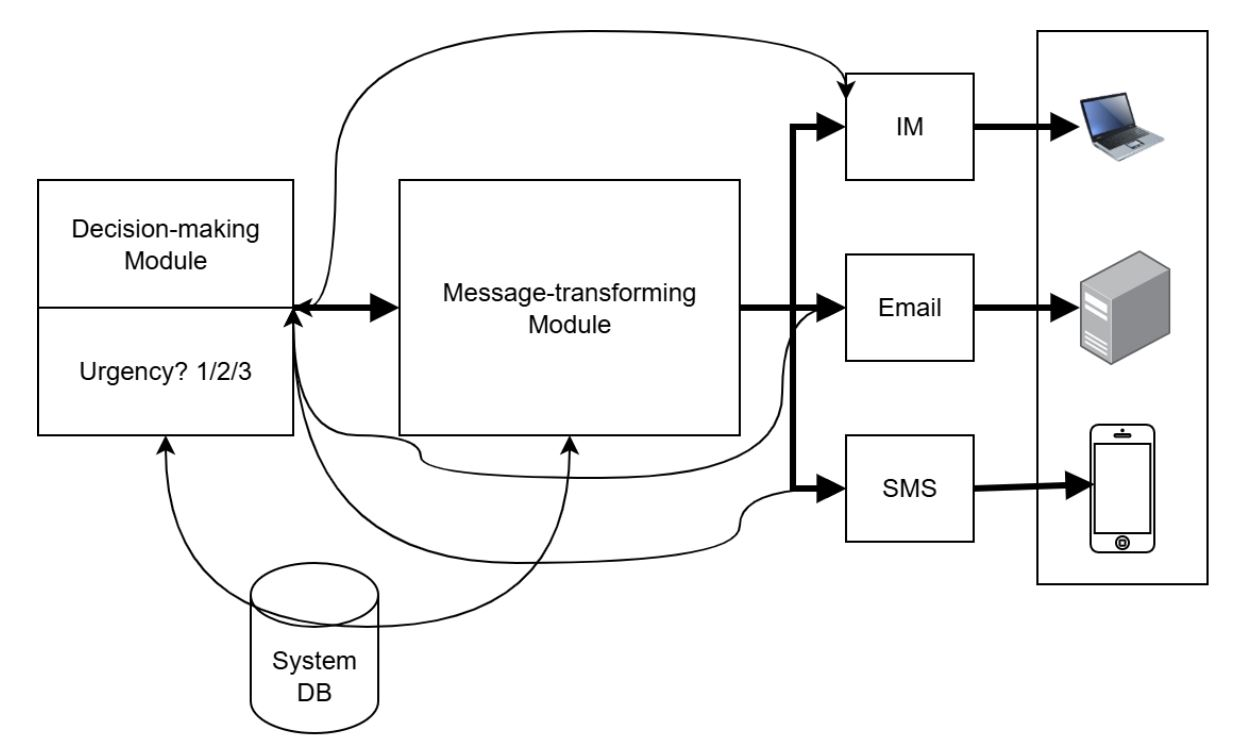
\includegraphics[width=0.45\textwidth]{liu2011-model.jpg}
  \caption{Integrated multi-channel messaging model supporting business collaboration \cite{liu2011}.}
  \label{fig:liu2011}
\end{figure}

\bibliographystyle{IEEEtran}
\bibliography{referencias}

\end{document}
